% --
% Neural Network Architectures

\section{Neural Network Architectures}\label{sec:nn_arch}
\thesisStateNotReady
All neural network architectures evaluated within this thesis are presented here.
The fundamental architectures were:
\begin{enumerate}
	\item Convolutional Neural Networks (CNN)
	\item Generative Adversarial Neural Networks (GAN)
	\item Wavenets
\end{enumerate}
%The term convolutional neural network here consists of all architectures consisting of at least one convolutional layer and the intention to simply classify each speech commands from each other. 
%Therefore the output of a convolutional net is of size of the number of individual speech commands and usually has some kind of probability distribution or energy equivalence.
CNNs were used for the classification of MFCC features and are therefore the main architecture within this thesis.
Generative models, such as GANs, are always worth to examine.
In this thesis, GANs were applied to evaluate network designs and their capability to generative convincing fakes and to use the trained feature maps in the convolutional layers for classifier networks as pre-trained weights.
Wavenets are compared to CNNs a completely different approach and use even raw audio samples as inputs.
Therefore for an online system, no MFCC features have to be calculated.
The saving of computations is evaluated as well as the performance compared to the CNN approach.

% --
% CNNs

\subsection{CNNs}\label{sec:nn_arch_cnn}
Three different CNN designs were evaluated, with the focus of the striding properties and therefore also the sizes of convolutional filters.
For one model the kernel size has the length of the frame (time) dimension of the input features and is therefore striding only in the MFCC (frequency) dimension.
The same holds for another model, but so that the kernel has the size of the feature dimension and therefore strides only in the frame dimension.
Also one traditional model is used, that does the strides as usual in both dimensions.
The naming of those models is as following:
\begin{itemize}
	\item \enquote{\texttt{trad}}: from \cite{Sainath2015} a traditional CNN network, striding in both dimensions.
	\item \enquote{\texttt{fstride4}}: from \cite{Sainath2015}, striding only in frequency dimension.
	\item \enquote{\texttt{conv-encoder-fc3}}: self designed model, striding only in frame dimension.
\end{itemize}
The network architecture of the traditional network (\texttt{trad}) is shown in \rfig{nn_arch_cnn_tra}.
% trad
\begin{figure}[!ht]
  \centering
    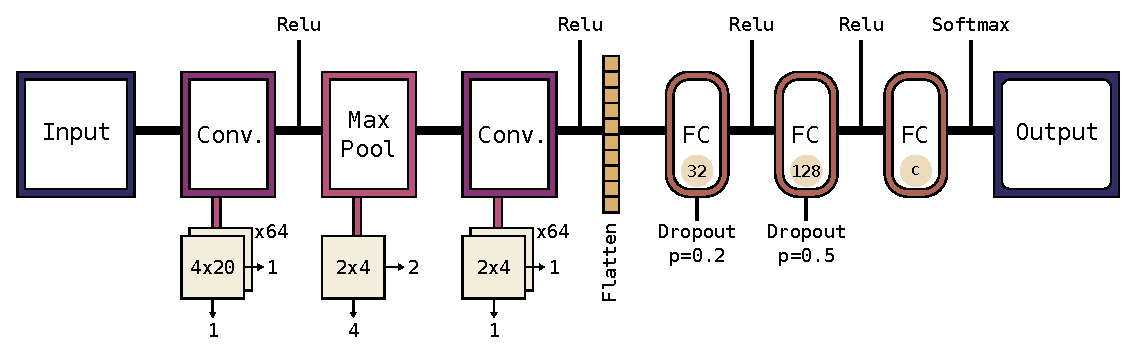
\includegraphics[height=0.2\textwidth]{./4_nn/figs/nn_arch_cnn_trad.eps}
  \caption{Traditional CNN network design from \cite{Sainath2015} named \texttt{trad}.}
  \label{fig:nn_arch_cnn_trad}
\end{figure}
\FloatBarrier
\noindent
The \texttt{trad} network consists of 2 convolutional layers and one max pooling layer in between.
The architecture was adapted from \cite{Sainath2015} as a baseline network and modified a bit in the kernel sizes, so that also reduced input features, for instance 12 MFCCs instead of 39 MFCC plus deltas and energies, can be computed with the same model.
The length of 20 frames in the first convolutional layer is reasonable and corresponse approximately to the length of a vowel sound.
Note that the \enquote{Flatten} layer simply flattens the output tensor of the last convolutional layers to 1-dimension, so that fully conected layers can be appended.
Dropout was used in the first two FC layers.
The last FC layer has $c$ nodes corresponding to $c$ output labels, depending on the amount of chosen key words in the vocabulary.

The \texttt{fstride4} model is shown in \rfig{nn_arch_cnn_fstride}
\begin{figure}[!ht]
  \centering
    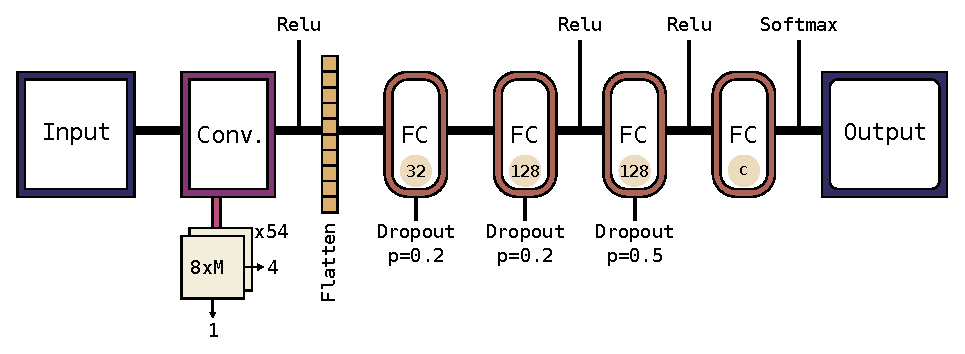
\includegraphics[height=0.2\textwidth]{./4_nn/figs/nn_arch_cnn_fstride.eps}
  \caption{Frequency striding CNN network design from \cite{Sainath2015} named \texttt{fstride4}.}
  \label{fig:nn_arch_cnn_fstride}
\end{figure}
\FloatBarrier
\noindent

The self designed \texttt{conv-encoder-fc3} model is shown in \rfig{nn_arch_cnn_conv-encoder-fc3}.
\begin{figure}[!ht]
  \centering
    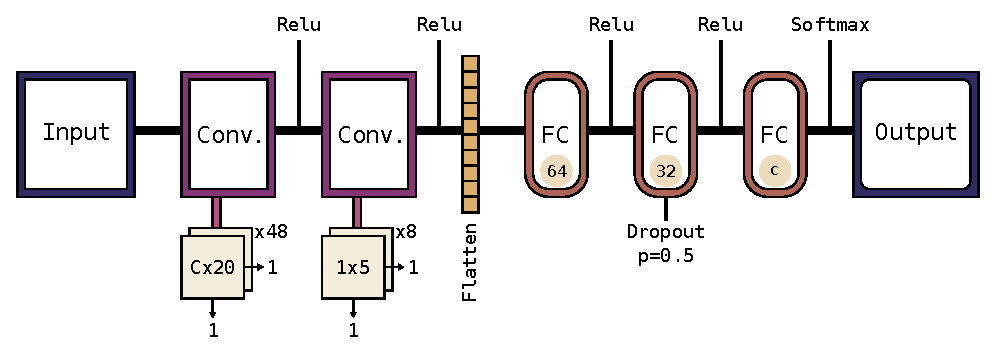
\includegraphics[height=0.2\textwidth]{./4_nn/figs/nn_arch_cnn_conv-encoder-fc3.eps}
  \caption{Self designed frame (time) striding CNN named \texttt{conv-encoder-fc3}.}
  \label{fig:nn_arch_cnn_conv-encoder-fc3}
\end{figure}
\FloatBarrier
\noindent


% --
% GANs

\subsection{GANs}\label{sec:nn_arch_gan}
t.b.d

\subsection{Wavenets}\label{sec:nn_arch_wavenet}
t.b.d

%With adversarial neural networks all architectures are meant, with at least two separate neural network architectures, e.g. a Discriminator and a Generator Network and the intention to outperform the other Network in a task where both play a game against each other.
%The word game is meant in the sense of game theory, where the goal is to find an equilibrium state of players competing against each other.
%An equilibrium state is usually found if all players are satisfied with the outcome.
%In this thesis the amount of players, or neural networks, is always two.
%An overview of all models is shown in \rtab{nn_arch_overview} with abbreviations in \rtab{nn_arch_abbreviation}.
%\begin{table}[ht!]
\begin{center}
\caption{Network Architectures Abbreviations}
\begin{tabular}{ M{2.5cm}  M{10cm} }
\toprule
\textbf{Abbreviations} & \textbf{Meaning}\\
\midrule
c[0-9] & convolutional layer with layer number\\
f[0-9] & feed forward fully connected layer with layer number\\
m[0-9] & max pooling layer layer with layer number\\
ch & input channel number for mfccs it is usually 1\\
fs & frame size (usually 50 -> 50ms)\\
ms & feature size (mfcc), depends on feature selection\\
cf & output number of last flattened convolutional layer\\
cl & number of class labels\\
\bottomrule
\label{tab:nn_arch_abbreviation}
\end{tabular}
\end{center}
\end{table}
\FloatBarrier
\noindent
%\begin{table}[ht!]
\begin{center}
\caption{Network Architectures Overview with reference names}
\begin{tabular}{ M{2.5cm}  M{2.1cm}  M{2.1cm} M{2.1cm} M{2.5cm}}
\toprule
%\multicolumn{4}{c}{\textbf{Feature Groups}} & \multicolumn{2}{c}{\textbf{Accuracy}} \\
\textbf{Reference name} & \textbf{Feature maps} & \textbf{Kernel sizes} & \textbf{Strides} & \textbf{Feed Forward} \\
\midrule
conv-trad & c1: (ch, 64) c2: (64, 64) & c1: (4, 20) mp: (2, 4) c2: (2, 4) & c1: (1, 1) mp: (2, 4) c2: (1, 1) & f1: (cf, 32) \quad f2: (32, 128) f3: (128, cl)\\
\midrule
conv-fstride & c1: (ch, 54) & c1: (8, fs) & c1: (4, 1) & f1: (cf, 32) \quad f2: (32, 128) \quad f3: (128, 128) \quad f4: (128, cl)\\
\midrule
conv-encoder-fc1 & c1: (ch, 48) \quad c2: (48, 8) & c1: (ms, 20) \quad c2: (1, 5) & c1: (1, 1) \quad c2: (1, 1) & f1: (cf, cl)\\
\midrule
conv-encoder-fc3 & c1: (ch, 48) \quad c2: (48, 8) & c1: (ms, 20) \quad c2: (1, 5) & c1: (1, 1) \quad c2: (1, 1) & f1: (cf, 64) \quad f2: (64, 32) \quad f3: (32, l)\\
\bottomrule
\label{tab:nn_arch_overview}
\end{tabular}
\end{center}
\end{table}
\FloatBarrier
\noindent


